\chapter{Validating a Graph Theoretic Screening Approach to Food Item Combinations}
\section{Abstract}
Tools from the mathematical field of graph theory potentially allow the consumer scientist to  efficiently analyze large numbers of combinations of food items, such as components on a salad.  In this study, we tested the validity of such an approach.  We began by asking subjects whether or not pairs of ingredients would be appropriate to combine on a salad.  Next, using graph theoretic methods, we predicted which combinations of 3-8 components should go together and, perhaps more importantly, which combinations should not.  Subjects were then asked whether or not particular combinations were appropriate to combine on a salad.  A paired Wilcoxon test between the predicted and non-predicted combinations was significant for all combination sizes.  

\section{Practical Applications}
A consumer driven graph theory methodology provides a screening tool to quickly and efficiently reduce a vast number of combinations of food items down to a reasonable number which can then be evaluated by the consumer scientist using suitability criteria together with more traditional tools.  In the case of salads, we screened over 1.7 million combinations and eliminated all but a handful as being unsuitable.  This methodology has potential in menu development, portfolio design and individual product formulations.  The advantage to the researcher is that the method can be inexpensively performed, is non-biased and is comprehensive.  This study validates the use of this approach in a particular screening application.

\section{Introduction}
The challenge of finding optimal combinations of food items, an important problem with effectively unlimited commercial applications, has been visited repeatedly with varying levels of success.  For instance, \citet{Eindhoven1959} observed that the prediction of peoples’ preferences for combinations of food items, such as menu items, was more complex than just a linear additivity of the preference for the individual items.  Factors such as texture, color and separation of items \citep{Eindhoven1959,Pilgrim1961}, context and consumer ethnicity \citep{Marshall2003,Niewind1986}, frequency of consumption \citep{Marshall2003} and hypo-additivity or the “a la carte” effect \citep{Lawless1994} have all been found to complicate this combinatorial effect.  In addition, there are considerable individual differences that lead to one’s hedonic feelings towards a particular food item.  Taste, over texture or appearance, is the strongest predictor of liking but this is by no means ubiquitous \citep{Moskowitz1995}.   Further, in \citet{Moskowitz1995}, overall liking was predicted poorly by liking of individual components (R\superscript{2} values of 0.4 – 0.7).  It follows that if immediate progress is to be made towards meeting this challenge, a simplification would be desirable, and it was in search of such a simplification that \citet{Worsley1984} had grade school students evaluate 780 pairwise combinations of food items and answer how well “the foods in each pair would go together to form a nice meal.”  

A classical approach to analyzing pairwise information is to employ multidimensional scaling (MDS); whether deterministic \citep{Schiffman1981} or probabilistic \citep{Ennis1988}; a method of creating visual perceptual maps from similarity data.  This MDS methodology has been extended with cluster analysis to find entrées, starches and desserts that were close to each other, and followed by a regression analysis to predict compatibility ratings of the three component meal from the ratings given to the component pairs \citep{Klarman1977}.  A modified just-about-right scale \citep{Johnson1987} can also be used to evaluate optimal pairs of food items, and in the case of a wine and cheese pairing the two anchors would be “cheese dominates excessively” and “wine dominates excessively” with an “ideal match” point in the center \citep{King2005}.  \citet{Niewind1986} used a novel dual-scaling analysis \citep{Nishisato1984}, rather than MDS to analyze pairwise similarity categories on 39 different side dishes with 4 different main items.  Dual scaling (also known as Correspondence Analysis or CA) provides a way of quantifying and testing for significant differences between categorical data, such as complex questionnaires.

Regression analysis adds predictive capabilities to meal acceptability combination data.  The regression equations typically take on some variation of this form, where meal acceptability data of the individual components predicts whole meal results \citep{Hedderley1995,Moskowitz1983,Turner1988}:

\begin{equation}
Whole Meal = \beta _{0} + \beta _1(Appetizer) + \beta _2(Entree) + \beta _3(Dessert)\
\nonumber
\end{equation}
	
Modifications to the regression equation have been applied to the application of cyclic menus by means of a squared coefficient \citep{Moskowitz1983} for time since last presentation.  One of the effects noted above for combinations of food items is that scores are not additive.  

A more complex regression based method is conjoint analysis, which presents whole product concepts containing multiple elements or effects (packaging design, suggested time of eating, flavors, etc.) \citep{Green1978}.  Multiple concepts containing presence or absence of multiple values or levels of each of the different effects are presented to each subject and are either rated on a scale or as a binary accept/reject.  Regression analysis is used to determine the individual worth of each element towards the entire concept, and the model can then be used to find the best performing combination of attributes \citep{Moskowitz2006a}.  Conjoint analysis is strongly influenced by the axioms presented by \citet{Luce1964} which set a mathematical groundwork for what \citet{Luce1964} called conjoint measurement and justified the breaking down and recombining of individual effects to create an overall model.  One of the criticisms of conjoint analysis is that the concepts presented to the subjects must be derived by the practitioner and elements combined in such a way as to make them all independent of each other in the subsequent analysis.  A conjoint analysis measurement containing multiple effects and multiple levels, therefore, can have hundreds or thousands of different concepts to present to a consumer, which is a mentally challenging task and also greatly dependent on the abilities of the practitioner to design a good test.

In this paper, we explore an alternative approach to tackling problems involving pairs and combinations based on recent advances in mathematics and computer science, specifically in the field of graph theory \citep{Ennisa,Ennis2010,Ennis2011}.   We will see that graph theory emphasizes connections between items, rather than attributes of the items themselves and thus provides a novel perspective to explore this area of perception.  In particular, \citet{Ennis2010} have proposed a consumer driven methodology utilizing graph theory to approach our original challenge of finding optimal combinations of food items.  The choice of individual items is extremely flexible; items can be individual flavors, ingredients, pizza toppings, components of a ready to eat meal, etc.  This method is not meant to replace existing methodology but instead is meant to complement methods already in use by helping researchers screen a potentially astronomical number of combinations down to a manageable number that can then be studied using existing tools.  For example, if a consumer packaged goods company is developing a new frozen pizza, has 25 pizza toppings at their disposal and is interested in pizzas with  between two and eight toppings, there are 1,807,755 possible pizzas to consider.  Traditional strategies employed for screening these hypothetical pizzas for additional consideration typically include: discussion among a small committee of people, previous sales data, or in some cases consulting a single individual who is deemed to be an expert.  But these strategies, with the exception of conjoint approaches, are rarely consumer driven.

The technique we investigate is one of asking for pairwise information regarding item compatibility.  From this pairwise information, such as that collected by \citet{Worsley1984} and mentioned earlier, we use techniques from graph theory to build larger combinations suitable for additional examination using existing tools.  A vast number of unsuitable combinations will be eliminated from consideration allowing us to avoid the problem size issues experienced by conjoint based approaches.  As a metric for suitability, we will use appropriateness \citep{Schutz1988}, a concept that stems out of the development that acceptance is unpredictable and is not a great predictor of consumption \citep{Sidel1972}. By analyzing combinations under appropriateness conditions, the graph theory method explored in this paper maximizes external validity, rather than using hedonic ratings as a surrogate for whether or not people will consume an item.  The idea is to gather appropriateness information for pairs of items and then use mathematical tools to find combinations of items that are fully pairwise appropriate.  This technique will allow us to produce a short list of combinations worthy of additional investigation.  But the question remains, “Is this graph theoretic technique actually effective in practice?”  In other words, “Is it true that screened-out combinations are generally of low quality while combinations that survive the screening process are generally of high quality?”.  The contributions of this paper are then two-fold.  In particular we show in this paper that for a particular product category that the answers to the above questions are both “yes.”  But, more generally and more importantly, we demonstrate through our example a process one might follow to verify that the graph theoretic screening technique we review is appropriate for other product categories.  Once this tool has been verified for a category, the time and cost savings provided by the use of graph theoretic screening are potentially great.  To this end, we begin by reviewing concepts from graph theory that we need to conduct our screening.  We then describe an experiment conducted in the fresh salad category before we present analysis demonstrating that, in this case, the screening technique was effective according to the criteria listed above.  

\section{Graph Theory}

The basic constructions of graph theory are straightforward.  A graph is a collection of objects called vertices \citep{Bollobaas1998} joined together with connections called edges.  See Figure~\ref{fig:exgraph} for an example of a graph with 8 vertices and 12 edges.  

\begin{figure}[h!]
\caption[Example graph.]{Graph with eight vertices and twelve edges.}
\centering

\includegraphics[width=0.6\textwidth]{./img/basic_graph.png}
\label{fig:exgraph}
\end{figure}

The study of graphs is typically fruitful in any endeavor in which items may be either related or not, such as electronic circuit design \citep{Bollobaas1998},  protein interactions \citep{Palla2005}, social network analysis \citep{Knoke2008} and internet search \citep{Brin1998}.  To illustrate the use of graph theory in the study of food item compatibility, we view a list of 25 salad toppings as 25 vertices on a graph.  In this case, we consider vertices to be connected exactly when the salad toppings are compatible.  Our challenge of finding compatible larger collections of salad toppings can then be translated into the graph theoretic challenge of finding larger collections of vertices that are fully interconnected.  Such collections of vertices are called cliques.  In the case of subject response data, if the three pairwise combinations of ingredients Apple-Carrot, Banana-Carrot and Apple-Banana are compatible, then the larger combination or clique Apple-Banana-Carrot is a predicted compatible combination.  However, if one of the three pairs is not compatible, such as Apple-Carrot, then the larger combination is not a predicted combination (nor is it a clique).  Figure~\ref{fig:exmaxclique} shows the same graph as in Figure~\ref{fig:exgraph} with all of the (maximal) cliques highlighted.  For our salad example, we hypothesize: 1) cliques represent potential successful salads and 2) non-cliques represent unsuccessful salads that can safely be removed from future consideration.  An experimental validation of this hypothesis is the topic of our next section.  

\begin{figure}[h!]
\caption[Example graph with maximal cliques]{Graph from Figure~\ref{fig:exgraph} with maximal cliques circled.}
\centering
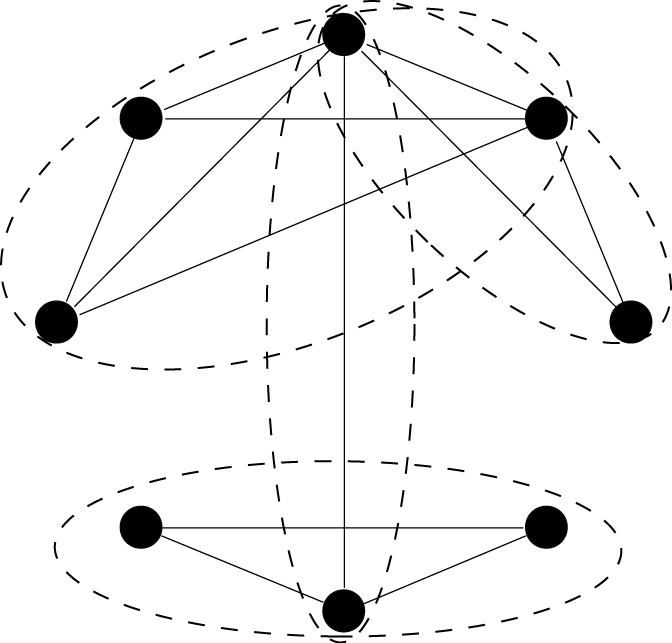
\includegraphics[width=0.6\textwidth]{./img/cliques.png}
\label{fig:exmaxclique}
\end{figure}

\section{Experimental Overview}
The study presented in this paper tests our hypothesis that combinations that are fully pairwise appropriate will be of high quality, i.e. will generally be judged as appropriate combinations, while those combinations that are not fully pairwise appropriate will be judged as inappropriate combinations.  In order to test this hypothesis, subjects were asked to provide appropriateness responses for pairwise combinations of 25 salad ingredients.  For each subject, their own complete set of cliques was formed.  Each subject was then asked whether or not it was appropriate to combine larger combinations of ingredients in a salad, using both cliques and random non-cliques for each size combination.  Our prediction was that the cliques method would perform significantly better than non-cliques.  

\section{Materials and Methods}
\subsection{Subjects}
105 responses were collected for an internet-based pre-survey (54 male), which gathered information on popular salad ingredients.  110 people participated in the main study.  Of those, 63 (22 male) were included in the final analysis.  The reason that 47 responses were excluded is because of the mathematical fact that if the subjects were too demanding or too accepting then there would not be enough cliques to test against the non-cliques, or conversely.  Thus, out of the 110 people whom completed the questionnaire, 63 continued on to the third part of the survey.  Prior to participation in the study, subjects were screened for regular salad consumption.  Subjects gave informed consent and this investigation was approved by the Cornell University Institutional Review Board.

\subsection{Pre-Survey Details}
The purpose of the pre-survey was to determine a list of 25 popular and familiar ingredients for use in the main survey.  An online questionnaire was developed which asked subjects to list the ingredients they would want in their favorite salad.  Panelists were recruited via department email lists and internet-based social networking websites. They were told that the salad included iceberg lettuce and no information was provided regarding a dressing.  Similar ingredients were combined (e.g. grilled chicken and chicken).  The final list is presented in Table~\ref{tab:salading}.


\begin{table}[h!b!p!]
\centering
\caption[25 popular salad ingredients]{25 popular salad ingredients determined from the pre-survey.  Similar ingredients were combined to produce a final list used in the subsequent supercombinatorial questionnaire.}
\begin{tabular}{cccc}
\toprule
\multicolumn{4}{c}{Ingredients} \\
\midrule
Tomatoes 		& 	Cucumbers 	& 	Carrots 	& 	Croutons 	\\
Bacon 			&	Blue Cheese 	& 	Spinach 	& 	Almonds 	\\
Chicken 		& 	Chickpeas 	& 	Feta Cheese 	& 	Onions 	\\
Sunflower Seeds 	& 	Black Olives 	& 	Broccoli 	&	Dried Cranberries \\
Hard-Boiled Egg 	& 	Cheddar 	& 	Mushroom 	& 	Avocado 	\\
Corn 			& 	Apples 		& 	Walnuts 	& 	Beets 		\\
Bell Peppers \\
\bottomrule
\label{tab:salading}
\end{tabular}
\end{table}

\subsection{Main Survey Details}
The survey for the second part of the study was conducted via computer at the sensory evaluation testing facility in the Cornell University Department of Food Science.  Custom software was developed by the Institute for Perception  to mimic a paper survey methodology with the addition of automated responses and analysis.  This allowed us to reduce panelist variability by performing the entire survey in a single session.  For Part 1, subjects were presented with the list of 25 ingredients, one at a time, and asked if under any circumstance they would consider consuming that ingredient on a salad.  If they chose no to any ingredient, that ingredient was removed from all subsequent parts of the survey for that subject.  

For Part 2, for each subject, all possible pairwise combinations from that subject’s remaining set of ingredients were generated.  For example, if a subjects selected 20 out of the 25 ingredients in Part 1, then 190 pairs were generated for Part 2.  The pairs were randomized in both overall order and with respect to presentation order within the pairs.  Subjects were asked, for each, to answer a YES/NO question as to whether or not they would consider the pair appropriate to combine together on a salad.  After appropriateness information regarding all pairs was collected, the software found cliques and non-cliques of sizes 3-8.  An equivalent number of cliques and non-cliques was presented for each, thus controlling for any size effect in the subsequent statistical analysis.  

For Part 3, the subjects were presented their own cliques and non-cliques (no more than 100 in each condition).  The order within and between sets of ingredients was again randomized.  In this part, as in Part 2, the subject was asked whether each combination was appropriate to combine on a salad and the software recorded the responses.  

\subsection{Data Analysis}
For the overall analysis we chose to combine maximal cliques and non-maximal cliques into a “clique” category.  When a combination was chosen by a subject to be appropriate, this was counted as compatible.  For each subject and for all subjects the total number of times a subject indicated that a combination was compatible for each of the two conditions – predicted compatible combinations (cliques) and predicted incompatible combinations (non-cliques)  - was counted.  The Wilcox paired rank sum test is a non-parametric test which can be used to evaluate whether or not two distributions of counts overlap or are separate.  This test was used to compare the two distributions being tested – predicted compatible vs. predicted incompatible – for all combination sizes.  All data analysis was performed in R 2.10.0 using the stats package.  

\section{Results}
\subsection{Pre-Survey}
The pre-survey successfully met our goals of determining a list of 25 popular salad ingredients, which are presented in Table~\ref{tab:salading}.  There were 161 unique ingredients ranging from obvious (mushrooms, cheddar cheese) to obscure (nacho flavored chips, sour cream).  The top 25 ingredients were agreed upon by at least 10 people at a minimum, with the tomatoes (\#1) being requested by 54 people.  

\subsection{Main Study}
To test our hypothesis that the graph theoretic screening is valid, we used pairwise compatibility ratings to predict larger combinations of food items by finding cliques.  Specifically, when cliques of 3+ food items were generated from pairwise compatibility ratings, we hypothesized that the proportion of people who would find the cliques appropriate would be significantly larger than the proportion of people who would find random non-cliques appropriate:  
\begin{align*}
 & H_o: P(clique) > P(non-clique)\\ 
 & H_a: P(clique) \neq P(non-clique)
\end{align*}

Figure~\ref{fig:saladgraph} shows a graph generated from the pairwise compatibility information from Panelist 1.  Each connection in the graph represents a “yes” response from the survey.  Immediately it is apparent that for this panelist some ingredients, such as bell peppers, are much more highly compatible than others, such as apples and avocado, represented by the number of edges in the graph connected to those nodes.  The clique finding algorithm found all fully interconnected combinations, or cliques, of 3 to 8 ingredients.  A subset of these maximal cliques, along with the tested non-maximal cliques and non-cliques is shown in Table~\ref{tab:ponesalad}.

\begin{figure}[h!]
\caption[A panelist's salad graph.]{Graph from a panelist showing pairwise connectivity information.  Apples and Bacon are less compatible than tomatoes and mushrooms.}
\centering

\includegraphics[width=0.9\textwidth]{./img/ind_super_pairgraph.png}
\label{fig:saladgraph}
\end{figure}

Table~\ref{tab:wilcoxsalad} shows the results from the overall Wilcoxon test used to assess predicted compatibility.  For every clique size, there is significant evidence in support of our hypothesis that the graph theoretic screening is valid.  It is particularly interesting to note that although one might expect less support for our hypothesis for larger combination sizes, given how far removed those combinations are from the pairwise information, we observe supporting evidence even for an eight component salad.   Out of the 63 subjects, only 3 chose more non-cliques than cliques as being compatible when summed over all combination sizes.  Proportions of people whom chose a greater number of cliques over non-cliques as being compatible are shown in Table~\ref{tab:propsalad}.

\begin{landscape}
\footnotesize
\begin{longtable}{lllllllll}
\caption[Panelist 1 Salad Combinations]{Salads for Panelist one with compatibility responses.} \\
\endfirsthead
\toprule
\endhead
\multicolumn{9}{c}{Continued on next page...} \\
\endfoot
\bottomrule
\endlastfoot
\bottomrule
\multicolumn{2}{l}{\bf Maximal Cliques} \\
\cmidrule(l){1-2}
Response & Item 1 & Item 2 & Item 3 & Item 4 & Item 5 & Item 6 & Item 7 & Item 8\\
\midrule
TRUE & Bell Pepper & Black Olive & Chicken & Cucumber & Blue Cheese & Broccoli  \\
TRUE & Chicken & Bacon & Mushroom & Bell Pepper \\
TRUE & Chicken & Bell Pepper & Mushroom & Tomato & Cucumber & Black Olive & Broccoli \\
\midrule
\multicolumn{2}{l}{\bf Non-Maximal Cliques} \\
\cmidrule{1-2}
Response & Item 1 & Item 2 & Item 3 & Item 4 & Item 5 & Item 6 & Item 7 & Item 8\\
\midrule
TRUE & Cucumber & Broccoli & Corn & Bell Pepper & Carrots & Tomato & Chicken & Mushroom \\
TRUE & Broccoli & Tomato & Onion & Corn & Chicken & Mushroom & Cucumber & Bell Pepper \\
TRUE & Corn & Cucumber & Chicken & Tomato & Bell Pepper & Carrot & Broccoli & Onion \\
TRUE & Chicken & Onion & Carrot & Cucumber & Mushroom & Tomato & Bell Pepper & Broccoli \\
TRUE & Tomato & Broccoli & Mushroom & Corn & Chicken & Cucumber & Onion & Carrots \\
TRUE & Bell Pepper & Chicken & Carrot & Mushroom & Cucumber & Onion & Broccoli & Corn \\
TRUE & Chicken & Tomato & Onion & Corn & Cucumber & Carrot & Mushroom & Bell Pepper \\
TRUE & Corn & Tomato & Bell Pepper & Broccoli & Carrot & Mushroom & Cucumber & Onion \\
TRUE & Carrot & Broccoli & Bell Pepper & Onion & Corn & Chicken & Mushroom & Tomato \\
\midrule
\multicolumn{9}{l}{\bf Non-Cliques} \\
\cmidrule{1-2}
Response & Item 1 & Item 2 & Item 3 & Item 4 & Item 5 & Item 6 & Item 7 & Item 8\\
\midrule
TRUE & Bell Pepper & Bacon & Avocado & Carrot & Cucumber & Blue Cheese & Onion & Black Olive \\
TRUE & Bell Pepper & Bacon & Avocado & Corn & Cucumber & Broccoli && \\
FALSE & Sun. Seeds & Blue Cheese & Bell Pepper & Carrot & Apple & Mushroom & Onion & Cucumber \\
FALSE & Cucumber & Onion & Corn & Black Olive &&&& \\
TRUE & Broccoli & Apple & Chicken & Tomato & Bacon & Carrot & Cucumber & \\
TRUE & Corn & Avocado & Onion & Carrot & Apple & Black Olive & Broccoli & Chicken \\
TRUE & Onion & Avocado & Black Olive & Corn & Blue Cheese & Tomato & Cucumber & Broccoli \\
TRUE & Corn & Broccoli & Chicken & Tomato & Blue Cheese & Bell Pepper & Tomato & Broccoli \\
FALSE & Tomato & Sun. Seeds & Corn & Mushroom & Onion & Apple & Chicken & Black Olive \\
TRUE & Onion & Mushroom & Black Olive & Cucumber & Blue Cheese & Bell Pepper & Tomato & Broccoli \\
FALSE & Blue Cheese & Bacon & Tomato & Carrot & Apple & Mushroom & Broccoli & Sun. Seeds \\
TRUE & Bacon & Bell Pepper & Cucumber & Sun. Seeds & Black Olive & Apple & Mushroom & Avocado
\label{tab:ponesalad}
\end{longtable}
\end{landscape}

\begin{table}[h!b!p!]
\caption[Wilcoxon Test Results]{Results summary from paired Wilcoxon signed rank test.  Counts of how many times subjects chose non-cliques were compatible were compared to counts of how many times subjects chose cliques to be compatible.  In all combination sizes tested, clique compatibilities were significantly higher than non-cliques compatibilities.}
\centering
\begin{tabular}{cccc}
\toprule
{\bf Combination Size} & {\bf P(clique)} & {\bf P(non-clique)} & {\bf Wilcox p-value} \\
\midrule
3 & 0.52 & 0.26 & 0.025 \\
4 & 0.54 & 0.28 & 0.023 \\
5 & 0.79 & 0.52 & 0.016 \\
6 & 0.90 & 0.46 & \textless 0.001 \\
7 & 0.79 & 0.55 & 0.006 \\
8 & 0.93 & 0.53 & \textless 0.001 \\
\bottomrule
\end{tabular}
\label{tab:wilcoxsalad}
\end{table}

\section{Discussion and Conclusion}
A graph theoretic approach to determining optimal food combinations is a novel approach that shows promise in addressing difficult problems in consumer research.  In particular, the graph theoretic technique for screening out inappropriate combinations described in this paper stands to augment existing techniques by allowing researchers to quickly and easily arrive at a small list of reasonable candidates that may then be examined using existing techniques.  In this paper we have presented results demonstrating the validity of a graph theoretic screening approach for the fresh salad category.  Showing that this approach is valid in other categories will be an important and necessary step in the investigation of these graph theoretic techniques.  The design presented in this paper, in which subjects were queried first regarding appropriateness of pairs of items and later regarding the appropriateness of larger combinations of items, both cliques and non-cliques, can be used to test the validity of graph theoretic screening in other product categories.  

As can be seen by Table~\ref{tab:propsalad}, some individuals do prefer non-cliques, and some predicted cliques were not compatible.   Thus it is possible that a good combination could be missed by this approach (Type II error), or a predicted combination could fail (Type I error).  However, this method does reduce the chance of both kinds of error.  Further manual screening of predictions is a recommended approach to help protect against Type I error.    

\begin{table}[h!b!p!]
\caption[Proportions of people whom preferred cliques over non-cliques to be compatible.]{Proportions of people who overall chose more cliques than non-cliques to be compatible for each tested combination size.}
\centering
\begin{tabular}{cc}
\toprule
{\bf Combination Size} & {\bf P(compatible)} \\
\midrule
3 & 0.82 \\
4 & 0.77  \\
5 & 0.77 \\
6 & 0.92 \\
7 & 0.75 \\
8 & 0.96  \\
\bottomrule
\end{tabular}
\label{tab:propsalad}
\end{table}

There are a number of potential improvements to the method.  Our compatibility response data are binomial (Yes/No).  Scaling of response data does offer an alternative which may increase sensitivity and reduce the number of subjects needed for stabilized results.  Another potential improvement would be to allow subjects to taste individual items during the test as desired to familiarize or re-familiarize themselves with the components, as this investigation operated under the assumption that everyone tested whom was a salad consumer was familiar with all of the items.

As a final point, it is worth noting that in our present study, we focused on whether or not graph theoretic screening is valid at an individual level since the cliques we presented subjects were based on their individual compatibility responses for pairs of items.  Testing whether or not graph theoretic screening is valid at a group level is an additional important step in this research program.  Such group level testing will be the topic of future research.    

\pagebreak
\renewcommand\bibname{{REFERENCES}} %  will print "REFERENCES" instead of "BIBLIOGRAPHY"
\phantomsection
\addcontentsline{toc}{section}{References} %  adds "REFERENCES" to the table of content
\bibliographystyle{apalike}
\bibliography{library_man}  % uses the references stored in Chapter1Radar.bib